\documentclass[aspectratio=169, xcolor=dvipsnames]{beamer}

%----------------------------------------------
% TEMA Y COLORES PERSONALIZADOS
%----------------------------------------------
\usetheme[progressbar=frametitle]{Madrid}% Tema claro, profesional
\usepackage{xcolor}
\definecolor{micolor}{RGB}{184, 45, 42} % rojo oscuro personalizado
\setbeamercolor{structure}{fg=micolor} % Color principal

% Cambiar colores de los títulos y bloques
\setbeamercolor{title}{fg=white}
\setbeamercolor{frametitle}{fg=white}
\setbeamercolor{section in toc}{fg=black}
\setbeamercolor{block title}{fg=white,bg=micolor}
\setbeamercolor{block body}{bg=white, fg=black}
\setbeamercolor{item}{fg=micolor}

%----------------------------------------------
% PAQUETES
%----------------------------------------------
\usepackage[utf8]{inputenc}
\usepackage[english]{babel}
\usepackage{graphicx}
\usepackage{amsmath, amsfonts, amssymb}
\usepackage{booktabs}
\usepackage{hyperref}
\usepackage{subcaption}
\usepackage{quantikz}
\usepackage{svg}
\usepackage{tikz}
\usepackage{adjustbox}
\usetikzlibrary{arrows.meta, positioning, shapes.geometric}

\setbeamertemplate{caption}[numbered]

\addtobeamertemplate{background}{
  \begin{tikzpicture}[remember picture,overlay]
    \node[opacity=0.09] at (current page.center) {
      
\includegraphics[width=0.4\paperwidth]{Logo_mqst.png}
    };
  \end{tikzpicture}
}{}

\usepackage[
  backend=biber,
  style=ieee,     % cita [1], [2], etc.
  sorting=none,      % orden por aparición
  doi=false,         % elimina DOI
  url=false,         % elimina URL
  isbn=false,        % elimina ISBN
  eprint=false       % elimina e-prints
]{biblatex}

\usepackage{amsthm}
\usepackage[framemethod=TikZ]{mdframed}

\newcounter{theo}[section]\setcounter{theo}{0}
\renewcommand{\thetheo}{\arabic{section}.\arabic{theo}}
\newenvironment{theo}[2][]{%
\refstepcounter{theo}%
\ifstrempty{#1}%
{}%
{\mdfsetup{%
innertopmargin=2cm,
singleextra={\node[anchor=west,xshift=5mm,rectangle,fill=micolor,inner sep=0.5mm] at (P-|O) %
{\hspace*{5pt}\strut 
\textbf{\textcolor{white}{Estimation Precision}}
\hspace*{5pt}
% Theorem~\thetheo:~#1\hspace*{5pt}
};}}%
}%
\mdfsetup{linecolor=micolor,%
linewidth=2pt,topline=true,%
innertopmargin=1.5Em,
}
\begin{mdframed}[]\relax%
\label{#2}}{\end{mdframed}}

\addbibresource{biblioGPT.bib}

%----------------------------------------------
% INFORMACIÓN DE LA PRESENTACIÓN
%----------------------------------------------
\title[AQMCoursework]{Shor’s 1994 Quantum Factoring Algorithm: History, Mathematics, and Simulations}
\author[Shor's Algorithm]{Amey Bhatuse \\
Sergio Castañeiras Morales \\
David González Lociga \\
José Ernesto Ramos Sánchez
}
\institute[]{\textbf{Advanced Quantum Mechanics} \\ Master in Quantum Science and Technology Barcelona}
\date{October 21, 2025}

%----------------------------------------------
% INICIO DEL DOCUMENTO
%----------------------------------------------
\begin{document}

\input{files/title}



%\begin{frame}{Index}
	\textcolor{blue}{Needed?}
    \textcolor{red}{NO.}
    \tableofcontents
\end{frame}
\begin{frame}{Introduction}
\begin{columns}[c]
    \begin{column}{0.55\textwidth}
        \centering
        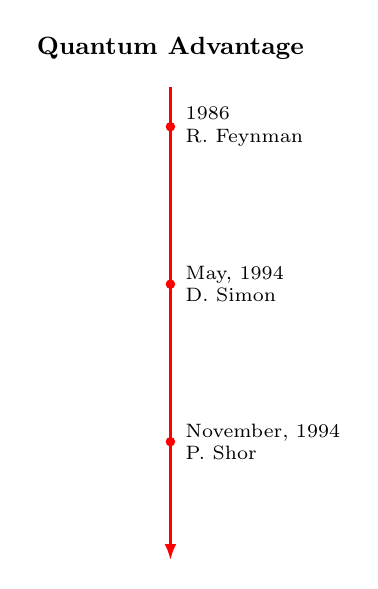
\begin{tikzpicture}[scale=1, % scale down to fit column
          timeline/.style={draw=red, thick, -{Latex[length=2mm]}}, 
          event/.style={circle, draw=red, fill=red, minimum size=3pt, inner sep=0.6pt}, 
          label/.style={font=\scriptsize, align=left}
        ]
        % Text above the timeline
        \node[font=\small\bfseries, align=center] at (0,6.5) {Quantum Advantage};
        % Línia temporal vertical (arrow down)
        \draw[timeline] (0,6) -- (0,0);

        % Esdeveniments
        \node[event] at (0,5.5) {};
        \node[label, right=2pt] at (0,5.5) {1986\\R. Feynman};

        \node[event] at (0,3.5) {};
        \node[label, right=2pt] at (0,3.5) {May, 1994\\D. Simon};

        \node[event] at (0,1.5) {};
        \node[label, right=2pt] at (0,1.5) {November, 1994\\P. Shor};

        \end{tikzpicture}
    \end{column}
    \begin{column}{0.45\textwidth}
        \centering
            \vspace{-0.2cm}
            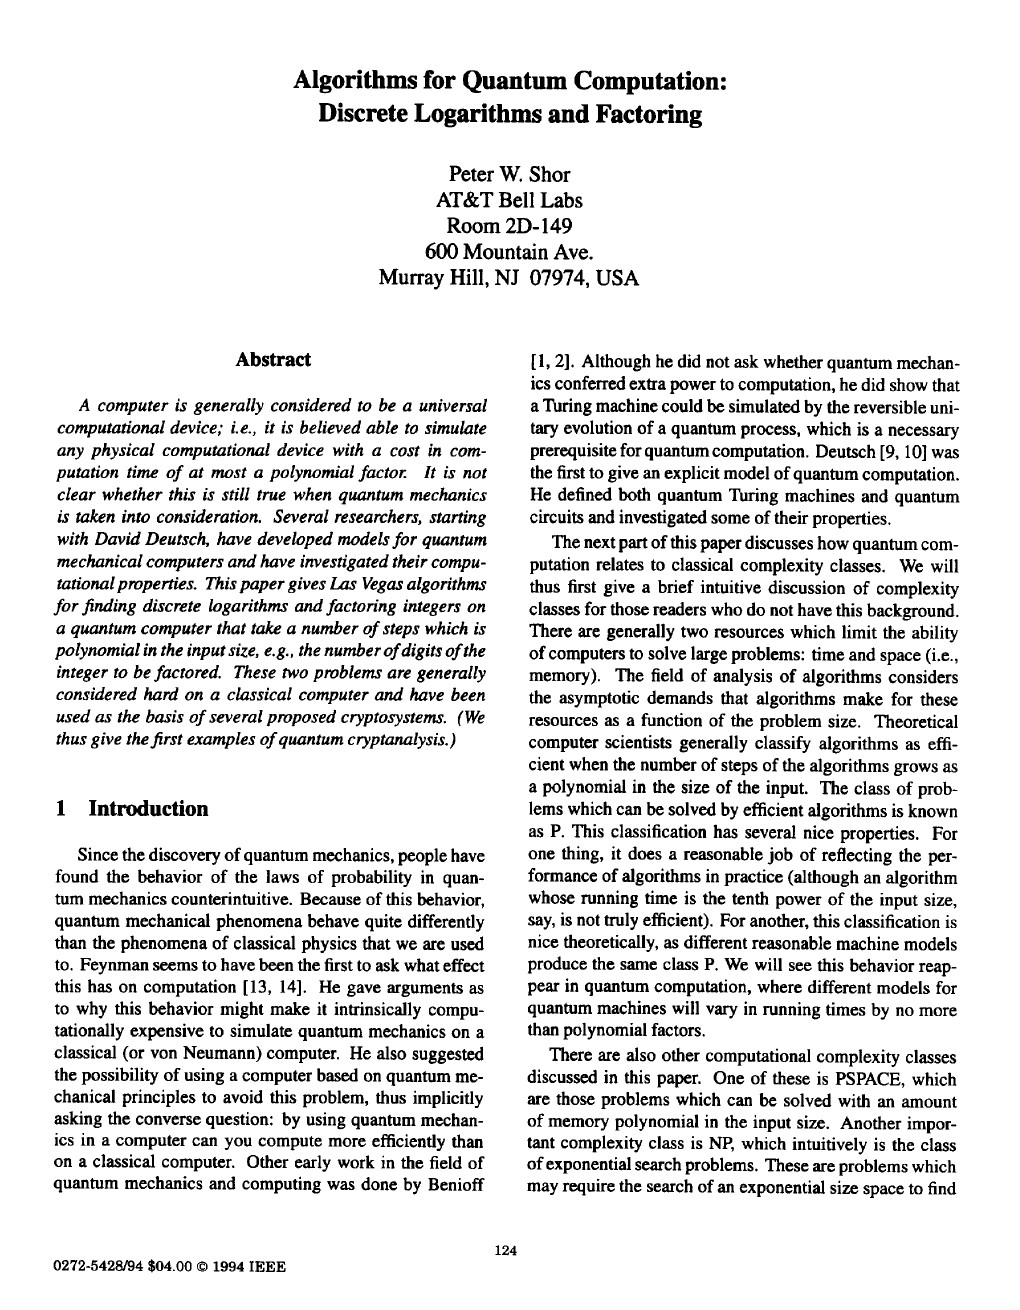
\includegraphics[width=0.9\linewidth, height=0.8
            \textheight, keepaspectratio]{Shor1994_pages-to-jpg-0001.jpg}
    \end{column}
\end{columns}
\end{frame}


\begin{frame}{Mathematical formulation}
\centering

\begin{definition}
    {\footnotesize
Given $n\in \mathbb{N}$, the multiplicative group of integers modulo $n$ is defined as
\[
\left(\mathbb{Z}/n\mathbb{Z}\right)^{*} 
= \{ [x] \in \mathbb{Z}/n\mathbb{Z} : \gcd(x,n)=1 \}.
\]
For example:
\[
\left(\mathbb{Z}/12\mathbb{Z}\right)^{*} 
= \{ [1],[5],[7],[11]\}.
\]
}
\end{definition}
\centering
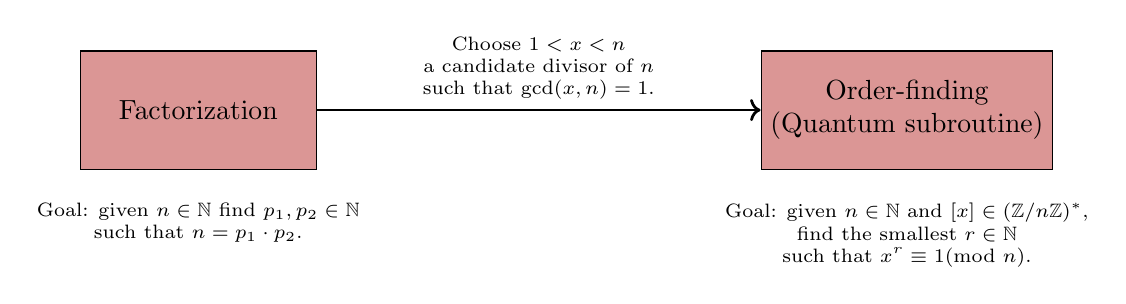
\begin{tikzpicture}[node distance=9cm, auto]

    % Left box
    \node[draw, rectangle, minimum width=3cm, minimum height=1.5cm, align=center, fill=micolor!50] (left) 
        {Factorization};
    
    % Text below left box
    \node[align=center, font=\scriptsize, below=0.3cm of left] (lefttext)
        {Goal: given $n\in\mathbb{N}$ find $p_1,p_2\in \mathbb{N}$\\ such that $n=p_1\cdot p_2.$ };

    % Right box
    \node[draw, rectangle, minimum width=3cm, minimum height=1.5cm, align=center, right of=left, fill=micolor!50] (right) 
        {Order-finding\\(Quantum subroutine)};
    
    % Text below right box
    \node[align=center, font=\scriptsize, below=0.3cm of right] (righttext)
        {Goal: given $n\in \mathbb{N}$ and $[x]\in\left(\mathbb{Z}/n\mathbb{Z}\right)^{*}$,\\ find the smallest $r\in \mathbb{N}$\\ such that $x^r\equiv 1 (\text{mod }n)$. };

    % Thick arrow connecting them with text
    \draw[->, line width=1pt] 
        (left) -- node[midway, above, font=\scriptsize, align=center] {Choose $1<x<n$\\ a candidate divisor of $n$\\ such that $\text{gcd}(x,n)=1$.} (right);

\end{tikzpicture}

Once $r$ is obtained, a classical algorithm finds a divisor of $n$!

\end{frame}


\begin{frame}
\begin{figure}
	\centering
\scalebox{0.70}{
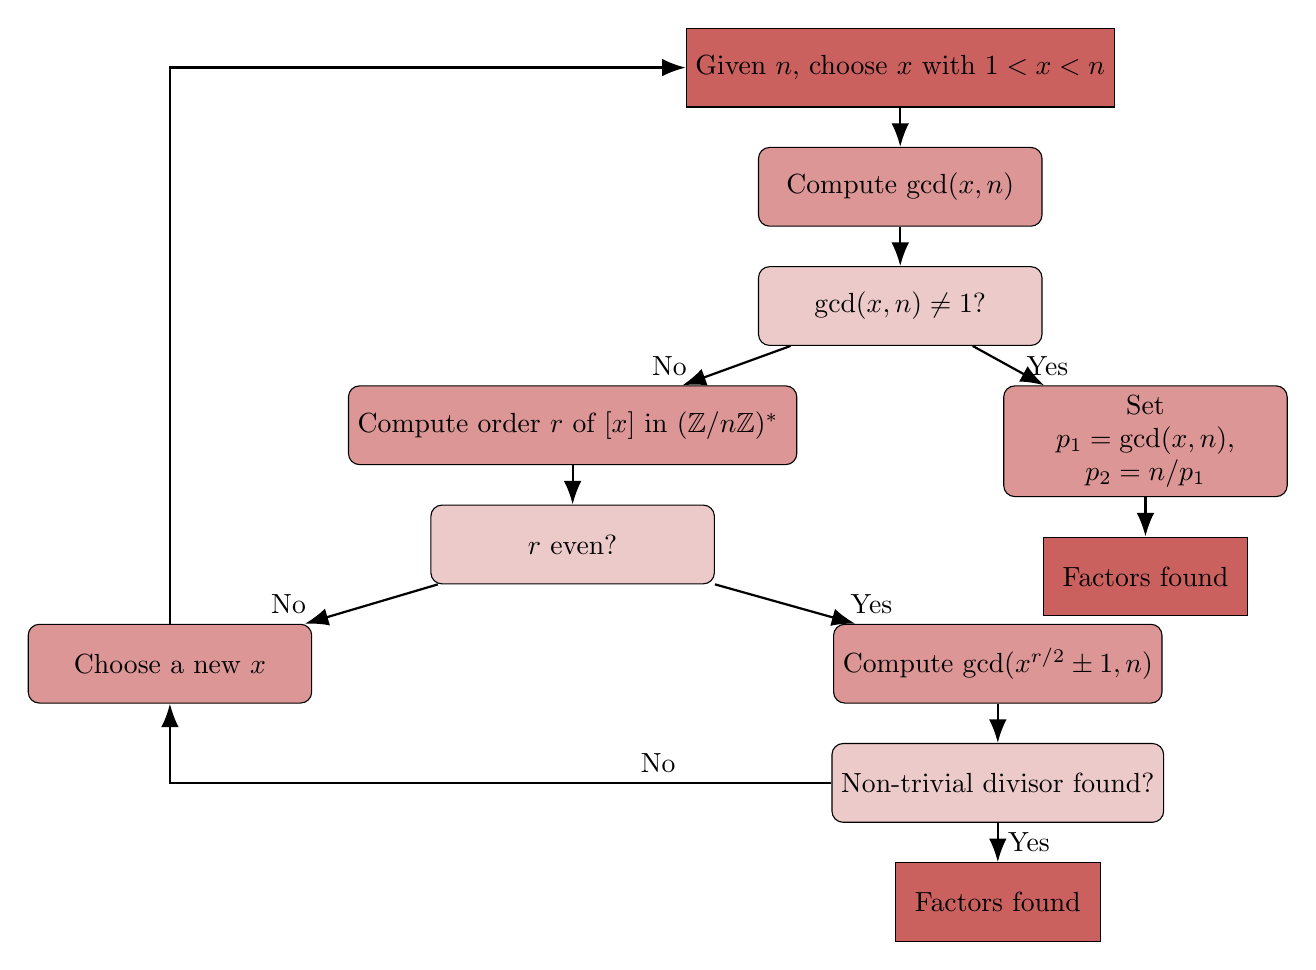
\begin{tikzpicture}[
    node distance=0.5cm and 0.5cm,
    every node/.style={align=center},
    startstop/.style={rectangle, draw, fill=micolor!75, minimum width=2.6cm, minimum height=1cm},
    process/.style={rectangle, rounded corners, draw, fill= micolor!50, minimum width=3.6cm, minimum height=1cm},
    decision/.style={rectangle, rounded corners, draw, fill=micolor!25, aspect=2, minimum width=3.6cm, minimum height=1cm},
    arrow/.style={-{Latex[length=3mm]}, thick}
]

% Nodes
% \node[startstop] (start) {Start};
\node[startstop] (input) {Given $n$, choose $x$ with $1 < x < n$};
\node[process, below=of input] (gcd) {Compute $\gcd(x,n)$};
\node[decision, below=of gcd] (checkgcd) {$\gcd(x,n) \neq 1$?};
\node[process, below right=of checkgcd, xshift=-1cm] (found) {Set \\ $p_1 = \gcd(x,n)$, \\ $p_2 = n / p_1$};
\node[startstop, below=of found] (end1) {Factors found};
\node[process, below left=of checkgcd, xshift=1cm] (order) {Compute order $r$ of $[x]$ in $(\mathbb{Z}/n\mathbb{Z})^*$ };
\node[decision, below=of order] (checkr) {$r$ even?};
\node[process, below left=of checkr, xshift=-1cm] (retry) {Choose a new $x$};
\node[process, below right=of checkr, xshift=1cm] (compute) {Compute $\gcd(x^{r/2} \pm 1, n)$};
\node[decision, below=of compute] (checkdiv) {Non-trivial divisor found?};
\node[startstop, below=of checkdiv] (end2) {Factors found};

% Connections
% \draw[arrow] (start) -- (input);
\draw[arrow] (input) -- (gcd);
\draw[arrow] (gcd) -- (checkgcd);
\draw[arrow] (checkgcd) -- node[right,xshift=0.1cm]{Yes} (found);
\draw[arrow] (found) -- (end1);
\draw[arrow] (checkgcd) -- node[left, xshift=-0.5cm]{No} (order);
\draw[arrow] (order) -- (checkr);
\draw[arrow] (checkr) -- node[left, xshift = -0.7cm]{No} (retry);
\draw[arrow] (retry) |- (input);
\draw[arrow] (checkr) -- node[right, xshift = 0.7cm]{Yes} (compute);
\draw[arrow] (compute) -- (checkdiv);
\draw[arrow] (checkdiv) -- node[right]{Yes} (end2);
\draw[arrow] (checkdiv) -| node[above, xshift = 6.2cm]{No} (retry);

\end{tikzpicture}
	}
\end{figure}
\end{frame}

\begin{frame}
\begin{figure}
	\centering
\scalebox{0.70}{
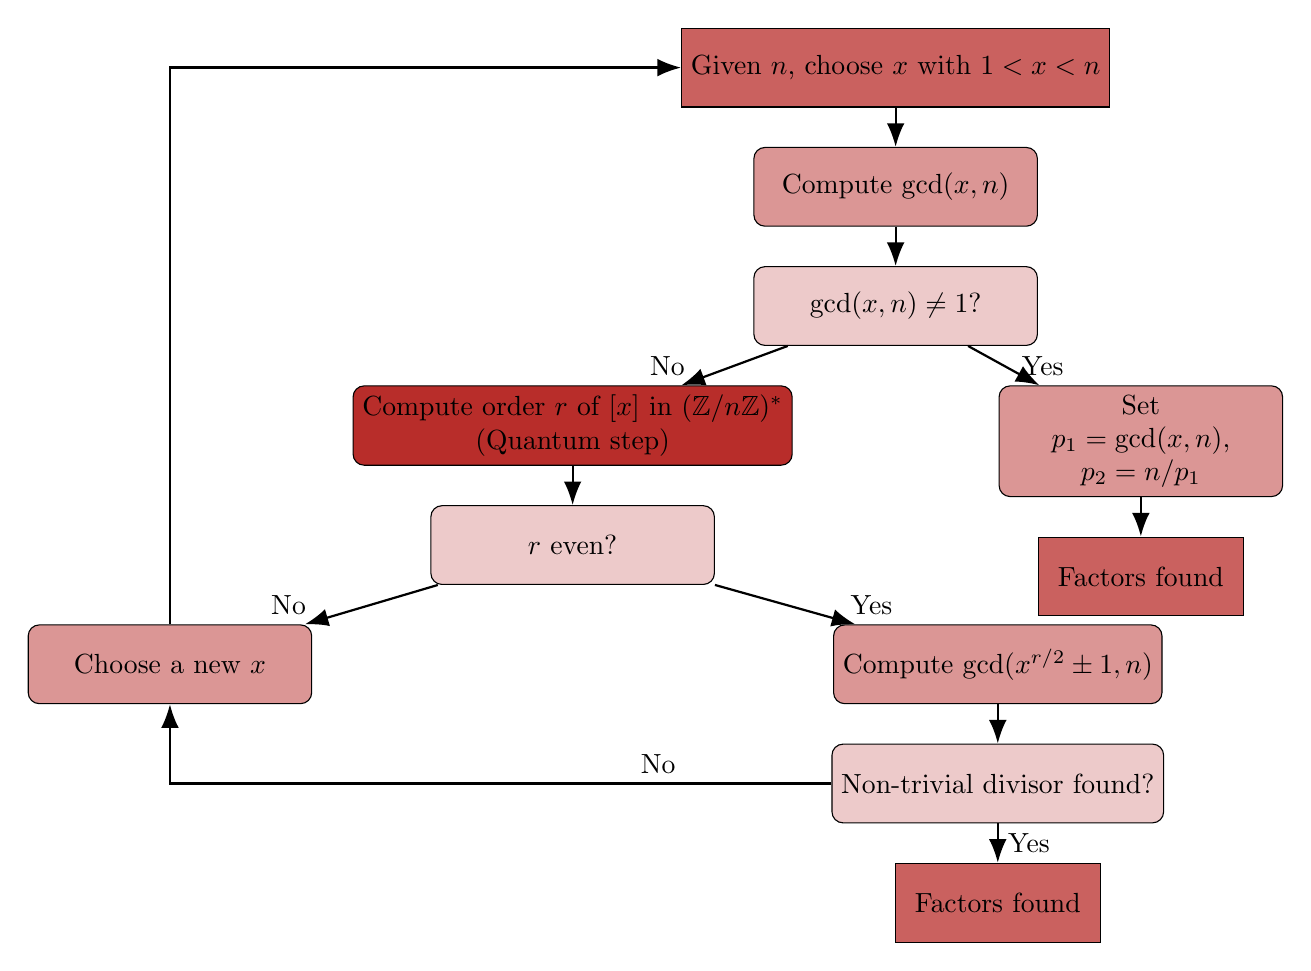
\begin{tikzpicture}[
    node distance=0.5cm and 0.5cm,
    every node/.style={align=center},
    startstop/.style={rectangle, draw, fill=micolor!75, minimum width=2.6cm, minimum height=1cm},
    quantum/.style={rectangle, rounded corners, draw, fill=micolor!100, minimum width=2.6cm, minimum height=1cm},
    process/.style={rectangle, rounded corners, draw, fill= micolor!50, minimum width=3.6cm, minimum height=1cm},
    decision/.style={rectangle, rounded corners, draw, fill=micolor!25, aspect=2, minimum width=3.6cm, minimum height=1cm},
    arrow/.style={-{Latex[length=3mm]}, thick}
]

% Nodes
% \node[startstop] (start) {Start};
\node[startstop] (input) {Given $n$, choose $x$ with $1 < x < n$};
\node[process, below=of input] (gcd) {Compute $\gcd(x,n)$};
\node[decision, below=of gcd] (checkgcd) {$\gcd(x,n) \neq 1$?};
\node[process, below right=of checkgcd, xshift=-1cm] (found) {Set \\ $p_1 = \gcd(x,n)$, \\ $p_2 = n / p_1$};
\node[startstop, below=of found] (end1) {Factors found};
\node[quantum, below left=of checkgcd, xshift=1cm] (order) {Compute order $r$ of $[x]$ in $(\mathbb{Z}/n\mathbb{Z})^*$ \\ (Quantum step)};
\node[decision, below=of order] (checkr) {$r$ even?};
\node[process, below left=of checkr, xshift=-1cm] (retry) {Choose a new $x$};
\node[process, below right=of checkr, xshift=1cm] (compute) {Compute $\gcd(x^{r/2} \pm 1, n)$};
\node[decision, below=of compute] (checkdiv) {Non-trivial divisor found?};
\node[startstop, below=of checkdiv] (end2) {Factors found};

% Connections
% \draw[arrow] (start) -- (input);
\draw[arrow] (input) -- (gcd);
\draw[arrow] (gcd) -- (checkgcd);
\draw[arrow] (checkgcd) -- node[right,xshift=0.1cm]{Yes} (found);
\draw[arrow] (found) -- (end1);
\draw[arrow] (checkgcd) -- node[left, xshift=-0.5cm]{No} (order);
\draw[arrow] (order) -- (checkr);
\draw[arrow] (checkr) -- node[left, xshift = -0.7cm]{No} (retry);
\draw[arrow] (retry) |- (input);
\draw[arrow] (checkr) -- node[right, xshift = 0.7cm]{Yes} (compute);
\draw[arrow] (compute) -- (checkdiv);
\draw[arrow] (checkdiv) -- node[right]{Yes} (end2);
\draw[arrow] (checkdiv) -| node[above, xshift = 6.2cm]{No} (retry);

\end{tikzpicture}
	}
\end{figure}
\end{frame}

\begin{frame}{Implementation of Shor's algorithm}
			\begin{figure}[H]
				\centering
\scalebox{0.70}{
\begin{quantikz}[row sep={0.7cm,between origins}, column sep=0.8cm]
        % First register (t qubits)
        \lstick{$\ket{0}_0$} & \gate{H} & \ctrl{4} & \qw & \qw & \qw & \gate[wires=4]{QFT^\dagger} & \meter{} \\
        \lstick{$\ket{0}_1$} & \gate{H} & \qw & \ctrl{3} & \qw & \qw &  & \meter{} \\
        \lstick{$\vdots$}\\
        \lstick{$\ket{0}_{t-1}$} & \gate{H} & \qw  & \qw & \qw & \ctrl{1} & \qw  & \meter{} \\
        % Second register (work register)
        \lstick{$\ket{1}$} & \qw & \gate{U^{2^{t-1}}} & \gate{U^{2^{t-2}}} & \dots   & \gate{U^{2^{0}}} & \qw & \rstick{$\ket{x^{j}º\bmod{n}}$}
\end{quantikz}
}
				\caption{Quantum circuit implementing Shor's algorithm.}
				\label{fig:shor_qc}
				
			\end{figure}


\begin{block}{Quantum Fourier Transform}
Let $\{\ket{k}\}_{k=0}^{N-1}$ be an orthonormal basis. We define the \textit{Quantum Fourier Transform} (QFT) as the unitary operation $U_{QFT}$ such that its action on the basis is,
\[U_{\text{QFT}}\ket{r}=\frac{1}{\sqrt{N}}\sum_{k=0}^{N-1}e^{i\frac{2\pi}{N}kr}\ket{k}.\]
\end{block}

\end{frame}

\begin{frame}{Implementation of Shor's algorithm}
		
			\begin{itemize}
				\item State before $QFT^{\dagger}$: $|\phi \rangle
				= \frac{1}{\sqrt{r2^t}} \sum_{j=0}^{2^t - 1} |j\rangle 
				\sum_{d=0}^{r-1} e^{i\frac{2\pi j d}{r}} |u_d\rangle
				= \frac{1}{\sqrt{2^t}} \sum_{j=0}^{2^t - 1} |j\rangle |x^j \bmod n\rangle$, where $|u_d\rangle$ are the eigenvectors of the unitary operator $U \, |y\rangle= |x y \,(\text{mod} \, n) \rangle$.
				
				\vspace{6pt}
				
				\item Final state: $|\psi \rangle
				= \frac{1}{\sqrt{r}}  \sum_{d=0}^{r-1} |\tilde{c}/q \rangle |u_d\rangle$, where $q=2^t$ and $\tilde{c}/q$ is an estimation of $d/r$ precise to $t$ bits. We will determine $d/r$ from the estimation $\tilde{c}/q$ using the continued fractions expansion.
			\end{itemize}
			\begin{figure}[H]
				\centering
\scalebox{0.90}{
\begin{quantikz}[row sep={0.7cm,between origins}, column sep=0.8cm]
        % First register (t qubits)
        \lstick{$\ket{0}_0$} & \gate{H} & \ctrl{4} & \qw & \qw & \qw & \gate[wires=4]{QFT^\dagger} & \meter{} \\
        \lstick{$\ket{0}_1$} & \gate{H} & \qw & \ctrl{3} & \qw & \qw &  & \meter{} \\
        \lstick{$\vdots$}\\
        \lstick{$\ket{0}_{t-1}$} & \gate{H} & \qw  & \qw & \qw & \ctrl{1} & \qw  & \meter{} \\
        % Second register (work register)
        \lstick{$\ket{1}$} & \qw & \gate{U^{2^{t-1}}} & \gate{U^{2^{t-2}}} & \dots   & \gate{U^{2^{0}}} & \qw & \rstick{$\ket{x^{j}º\bmod{n}}$}
\end{quantikz}
}
				\caption{Quantum circuit implementing Shor's algorithm.}
				\label{fig:shor_qc}
				
				
			\end{figure}
		
		
	\end{frame}

\begin{frame}{Implementation of Shor's algorithm}

% % \newcounter{theo}[section]
% \newenvironment{theo}[1][]{%
% % \stepcounter{theo}%
% % \ifstrempty{#1}%
% % {
% \mdfsetup{%
% frametitle={%
% \tikz[baseline=(current bounding box.east),outer sep=0pt]
% \node[anchor=east,rectangle,fill=blue!20]
% {\strut Theorem~\thetheo};}}
% % }%

% {\mdfsetup{%
% frametitle={%
% \tikz[baseline=(current bounding box.east),outer sep=0pt]
% \node[anchor=east,rectangle,fill=blue!20]
% {\strut Estimation Precision};}}%
% }%

% \mdfsetup{innertopmargin=10pt,linecolor=blue!20,%
% linewidth=2pt,topline=true,
% frametitleaboveskip=\dimexpr−\ht\strutbox\relax,}

% \begin{mdframed}[]\relax%
% % }\
% {\end{mdframed}}}

% \begin{theo}
%     Nice
% \end{theo}

% \newenvironment{theo}[1][]
% {
% \mdfsetup{%
% frametitle={%
% \tikz[baseline=(current bounding box.east),outer sep=2pt]
% \node[anchor=east,rectangle,fill=red]
% {\strut Estimation Precision};}}

% \mdfsetup{innertopmargin=10pt,linecolor=red,%
% linewidth=2pt,topline=true,
% frametitleaboveskip=\dimexpr−\ht\strutbox\relax,}

% {
% \begin{mdframed}
% % \relax%
% Nice
% \end{mdframed}
% }
% }


% \textbf{Estimation Precision}
    
% \[
% \mathbb{P}(\tilde{c})=\frac{1}{r2^{2t}}\sum_{d=0}^{r-1} \frac{\sin^2\left(\pi \left( \frac{d}{r}2^t -  \tilde{c} \right) \right)}{\sin^2\left(\pi \left( \frac{d}{r} -  \frac{\tilde{c}}{2^t} \right) \right)}
% \]



%\begin{theo}[yes]{}
%\[
%\mathbb{P}(\tilde{c})=\frac{1}{r2^{2t}}\sum_{d=0}^{r-1} \frac{\sin^2\left(\pi \left( \frac{d}{r}2^t -  \tilde{c} \right) \right)}{\sin^2\left(\pi \left( \frac{d}{r} -  \frac{\tilde{c}}{2^t} \right) \right)}
%\]
%!TEX encoding = UTF-8 Unicode\end{theo}

\begin{block}{Probability distribution}
The probability of measuring $\tilde{c}/q$ is calculated in the Quantum Phase Estimation (QPE) algorithm and it is given by,
\[
\mathbb{P}(\tilde{c})=\frac{1}{r2^{2t}}\sum_{d=0}^{r-1} \frac{\sin^2\left(\pi \left( \frac{d}{r}2^t -  \tilde{c} \right) \right)}{\sin^2\left(\pi \left( \frac{d}{r} -  \frac{\tilde{c}}{2^t} \right) \right)}.
\]
\end{block}

\end{frame}

	\begin{frame}{Example. Factoring $n$=55}
	\begin{itemize}
		\item We will begin by choosing $x=2$, which is coprime to $n=55$. 
	\end{itemize}
	
	\begin{block}{How many qubits should we use?}
	To ensure that we can find $d/r$ via the continued fractions expansion, we need at least,
	\begin{equation*}
		t=2L+1,
	\end{equation*}
	with $L=\lceil \log_2(n) \rceil$.
	\end{block}	
	
	\begin{itemize}
		\item In our example, $L=6$ and we need at least $t=13$ qubits.
	\end{itemize}
	
	
	\end{frame}

\begin{frame}{Example. Factoring $n=55$}
    \href{https://github.com/SirSergi0/AQM\_Coursework\_Group8}{\textcolor{blue}{\underline{Qiskit Code}}}
    
    \begin{figure}[t]
    \centering
    
\includegraphics[width=0.45\textwidth]{files/images/FractionsPlotBinaryN55n_count13.jpg}
    \caption{Comparison of results from running Shor's algorithm on N = 55 for t=13 and $2^{14}$ iterations with the plot for the analytical formula for estimation precision}
    \label{fig:plot_d_r}
\end{figure}
\end{frame}

\begin{frame}
    {Example. Factoring $n=55$}
	In Table \ref{tab:table} we illustrate the classical treatment for some of the most probable results $\tilde{c}/q$ of the quantum subroutine:

	\begin{table}[H]
		\centering
		\begin{tabular}{c c c c}
			\hline
			$\tilde{c}/q$ & $d/r$ & $r$ & Relative frequency  \\ 
			\hline
			0.04993 & 1/20 & 20 & 0.029 \\ 
			0.09998 & 1/10 & 10 & 0.045 \\ 
			0.80005 & 4/5  & 5  & 0.029 \\ 
			0.25000 & 1/4  & 4  & 0.049  \\ 
			\hline
		\end{tabular}
		\caption{Simulation results of $\tilde{c}/q$ with their corresponding relative frequency, the resulting $d/r$ from continued fractions expansion and the estimation for $r$.}
				\label{tab:table}
	\end{table}
	
	\begin{itemize}
		\item One source of failure is that $d$ and $r$ might share common factors that simplify. This occurs precisely when the results $r=10,5,4$ are obtained.
	\end{itemize}
\end{frame}

\begin{frame}{Example. Factoring $n = 55$}
		Since the correct order $r=20$ is even, we can continue with the classical part of the algorithm.
		\begin{block}{Classical post-processing in Shor's algorithm}
	
		\[
		\colorbox{red!15}{$r = 20$}
		\;\Rightarrow\;
		\begin{cases}
			\gcd(2^{20/2}-1,\,55) = 11\\[4pt]
			\gcd(2^{20/2}+1,\,55) = 5
		\end{cases}
		\;\Rightarrow\;
		\colorbox{red!15}{$55 = 5 \times 11$}
		\]
		\end{block}
	\end{frame}

\begin{frame}{Conclusions}
  \begin{itemize}
    \item We have reviewed Shor's original paper and detailed the mathematical framework underneath the algorithm. 
    \item We have reproduced Shor’s analytical probability distribution formulation of measuring $\frac{\tilde{c}}{q}$.
    \item We have verified the analytical expression  with numerical results from a practical implementation of the algorithm using the Qiskit framework. 
\end{itemize}  
\end{frame}
%----------------------------------------------
\section*{Thank you}

% \begin{frame}
%     \centering
%     \Huge{\textbf{Thank you for your attention!}}\\
%     \vspace{1cm}
% \end{frame}

\begin{frame}
    \centering
    \Huge{\textbf{Thank you for your attention!}}\\
    \vspace{1cm}
\end{frame}

%\begin{frame}[allowframebreaks]{References}
%  \scriptsize
%  \printbibliography
%\end{frame}

\begin{frame}
    \centering
    \vspace{1cm}
    {\fontsize{24pt}{24pt}\selectfont \textbf{Backup slides}}
\end{frame}

\begin{frame}{QFT circuit implementation}
    \begin{figure}
\centering
\scalebox{0.7}{ % full size, no shrinking needed
\begin{quantikz}[
  row sep=0.5cm, 
  column sep=0.4cm, 
  /tikz/every label/.append style={font=\small},
  /tikz/every gate/.append style={minimum width=0.5cm, minimum height=0.35cm, inner sep=0pt, font=\normalsize}
]
\lstick{$\ket{k_1}$} & \gate{H} & \gate{R_2} & {\hspace{0.1cm}\dots\hspace{0.1cm}} & \gate{R_{n-1}} & \gate{R_n} & \qw & \qw & \qw & \qw & \qw & \qw & \qw & \qw & \qw & \rstick{$\ket{0}+e^{2\pi i0.k_1\dots k_n}\ket{1}$}\\
\lstick{$\ket{k_2}$} & \qw & \ctrl{-1} & {\hspace{0.1cm}\dots\hspace{0.1cm}} & \qw & \qw & \gate{H} & {\hspace{0.1cm}\dots\hspace{0.1cm}} & \gate{R_{n-2}} & \gate{R_{n-1}}& {\hspace{0.1cm}\dots\hspace{0.1cm}} & \qw & \qw  & \qw & \qw & \rstick{$\ket{0}+e^{2\pi i0.k_2\dots k_n}\ket{1}$}\\
\lstick{$\vdots$} \\ 
\lstick{$\ket{k_{n-1}}$} & \qw & \qw & \qw & \ctrl{-3} & \qw & \qw & \qw & \ctrl{-2} &  \qw & {\hspace{0.1cm}\dots\hspace{0.1cm}}  &\gate{H} &\gate{R_2} & \qw & \qw & \rstick{$\ket{0}+e^{2\pi i0.k_{n-1}k_n}\ket{1}$}\\
\lstick{$\ket{k_n}$} & \qw & \qw & \qw & \qw & \ctrl{-4} & \qw & \qw & \qw & \ctrl{-3} & {\hspace{0.1cm}\dots\hspace{0.1cm}} & \qw & \ctrl{-1} & \gate{H} & \qw & \rstick{$\ket{0}+e^{2\pi i0.k_n}\ket{1}$}\\
\end{quantikz}}

% 
\includegraphics[
% width=38cm, 
% height=10cm]{fig_QFT.pdf}

% }
\caption{Quantum circuit implementing the Quantum Fourier Transform (QFT). 
The output states are shown unnormalized (the $1/\sqrt{2}$ factors are omitted). 
Controlled phase shift gates $CR_k$ are represented by phase shift gates $R_k$ acting on the target qubit, 
with filled dots indicating their respective control qubits. Notice how by reading the output qubits downwards, we obtain the QFT in the reversed order, so a final SWAP gate is required in order to obtain the desired result.}
\label{fig:qft}
\end{figure}
\end{frame}


\begin{frame}{Precision}
\begin{block}{How does the precision scale with $t$?}
If we use $t$ qubits in the first register, 
\begin{equation*}
t=2L + 1 + \left\lceil \log_2\left(2+\frac{1}{2\epsilon}\right) \right\rceil,
\end{equation*}
we will obtain an estimate $\tilde{c}/q$ of the phase $d/r$ accurate to $2L+1$ bits with probability at least $(1-\epsilon)/r$.
\end{block}

\end{frame}


\end{document}
